\chapter{Структуры}

\begin{lstlisting}[caption={\text{Структура FILE}}]
typedef struct _IO_FILE FILE;
struct _IO_FILE
{
	int _flags;		/* High-order word is _IO_MAGIC; rest is flags. */
	
	/* The following pointers correspond to the C++ streambuf protocol. */
	char *_IO_read_ptr;	/* Current read pointer */
	char *_IO_read_end;	/* End of get area. */
	char *_IO_read_base;	/* Start of putback+get area. */
	char *_IO_write_base;	/* Start of put area. */
	char *_IO_write_ptr;	/* Current put pointer. */
	char *_IO_write_end;	/* End of put area. */
	char *_IO_buf_base;	/* Start of reserve area. */
	char *_IO_buf_end;	/* End of reserve area. */
	
	/* The following fields are used to support backing up and undo. */
	char *_IO_save_base; /* Pointer to start of non-current get area. */
	char *_IO_backup_base;  /* Pointer to first valid character of backup area */
	char *_IO_save_end; /* Pointer to end of non-current get area. */
	
	struct _IO_marker *_markers;
	
	struct _IO_FILE *_chain;
	
	int _fileno;
	int _flags2;
	__off_t _old_offset; /* This used to be _offset but it's too small.  */
	
	/* 1+column number of pbase(); 0 is unknown. */
	unsigned short _cur_column;
	signed char _vtable_offset;
	char _shortbuf[1];
	
	_IO_lock_t *_lock;
	#ifdef _IO_USE_OLD_IO_FILE
};
\end{lstlisting}

\begin{lstlisting}[caption={\text{Структура stat}}]
	struct stat
  {
    /* These are the members that POSIX.1 requires.  */

    __mode_t st_mode;		/* File mode.  */
#ifndef __USE_FILE_OFFSET64
    __ino_t st_ino;		/* File serial number.  */
#else
    __ino64_t st_ino;		/* File serial number.	*/
#endif
    __dev_t st_dev;		/* Device containing the file.  */
    __nlink_t st_nlink;		/* Link count.  */

    __uid_t st_uid;		/* User ID of the file's owner.  */
    __gid_t st_gid;		/* Group ID of the file's group.  */
#ifndef __USE_FILE_OFFSET64
    __off_t st_size;		/* Size of file, in bytes.  */
#else
    __off64_t st_size;		/* Size of file, in bytes.  */
#endif

    __time_t st_atime;		/* Time of last access.  */
    __time_t st_mtime;		/* Time of last modification.  */
    __time_t st_ctime;		/* Time of last status change.  */

    /* This should be defined if there is a `st_blksize' member.  */
#undef	_STATBUF_ST_BLKSIZE
  };
\end{lstlisting}

\chapter{Программа 1} 

\section{Однопоточная реализация}

\begin{lstlisting}[caption={\text{Программа №1}}]
#include <stdio.h>
#include <fcntl.h>

#define BUF_SIZE 20
#define FILENAME "alphabet.txt"

int main()
{
  int fd = open(FILENAME, O_RDONLY);

  FILE* fs1 = fdopen(fd, "r");
  char buff1[BUF_SIZE];
  setvbuf(fs1, buff1, _IOFBF, BUF_SIZE);

  FILE* fs2 = fdopen(fd, "r");
  char buff2[BUF_SIZE];
  setvbuf(fs2, buff2, _IOFBF, BUF_SIZE);

  int flag1 = 1, flag2 = 2;
  while(flag1 == 1 || flag2 == 1)
  {
    char c;

    flag1 = fscanf(fs1, "%c", &c);
    if (flag1 == 1)
    {
      fprintf(stdout, "%c", c);     
    }

    flag2 = fscanf(fs2, "%c", &c);
    if (flag2 == 1)
    {
      fprintf(stdout, "%c", c); 
    }
  }

  return 0;
}
\end{lstlisting}

\textbf{Вывод программы}

\begin{lstlisting}
	aubvcwdxeyfzghijklmnopqrst
\end{lstlisting}

\section{Многопоточная реализация}

\begin{lstlisting}
	#include <fcntl.h>
#include <pthread.h>
#include <stdio.h>

#define BUF_SIZE 20
#define FILENAME "alphabet.txt"

void* thread1(void *args) 
{
  int* fd = (int*)args;
  FILE* fs1 = fdopen(*fd, "r");
  char buff1[BUF_SIZE];
  setvbuf (fs1, buff1, _IOFBF, BUF_SIZE);

  int flag = 1;
  char c;
  while ((flag = fscanf(fs1, "%c", &c)) == 1)
  {
    fprintf(stdout, "%c", c);
  }

  return NULL;
}

void* thread2(void* args) 
{
  int* fd = (int*)args;
  FILE* fs2 = fdopen(*fd, "r");
  char buff2[BUF_SIZE];
  setvbuf ( fs2, buff2, _IOFBF, BUF_SIZE);

  int flag = 1;
  char c;
  while ((flag = fscanf(fs2, "%c", &c)) == 1) 
  {
    fprintf(stdout, "%c", c);
  }

  return NULL;
}

int main() 
{
  pthread_t t1, t2 ;

  int fd = open(FILENAME, O_RDONLY);

  pthread_create(&t1, NULL, thread1, &fd);
  pthread_create(&t2, NULL, thread2, &fd);

  pthread_join(t1, NULL);
  pthread_join(t2, NULL); 

  return 0 ;
}

\end{lstlisting}

\textbf{Вывод программы на разных запусках}

\begin{lstlisting}
	abcdefghijklmnopqrstuvwxyz
	abcdefuvwxyzghijklmnopqrst
	abcdeuvwxyzfghijklmnopqrst
\end{lstlisting}

\section{Пояснение}
В программе файл открывается 1 раз системным вызовом \texttt{open()},  который возвращает дескриптор файла типа int в usermode. Возвращенный номер fd~---~индекс дескриптора открытого файла в таблице дискрипторов открытых файлов процесса.
	
 Затем 2 раза вызывается функция \texttt{fdopen()} библиотеки stdio, которая создаёт указатель на структуру \texttt{FILE}, определенную с помощью define на базе \texttt{struct \_IO\_FILE}. 
 
 Функции \texttt{fdopen()} нужно передать возвращённый из \texttt{open()} дескриптор fd. Поле \_fileno в \texttt{struct \_IO\_FILE} содержит номер этого дескриптора.
	
 Функция \texttt{setvbuf()} устанавливает размер буфера 20 байт.
	
 При первом вызове функции \texttt{fscanf()} в цикле (для fs1) buff1 будет заполнен полностью~---~первыми 20 символами (буквами латинского алфавита). f\_pos в структуре \texttt{struct\_file} открытого файла увеличится на 20.
	
 При втором вызове \texttt{fscanf()} в цикле (для fs2) буфер buff2 будет заполнен оставшимися 6 символами (начиная с f\_pos, изменённого после 1-ого вызова \texttt{fscanf()}).
 
 В случае многопоточной реализации потоки выполняются с разной скоростью,  поэтому символы перемешаются.
 
 \begin{table}[H]
	\centering
	\begin{tabular}{p{1\linewidth}}
		\centering
		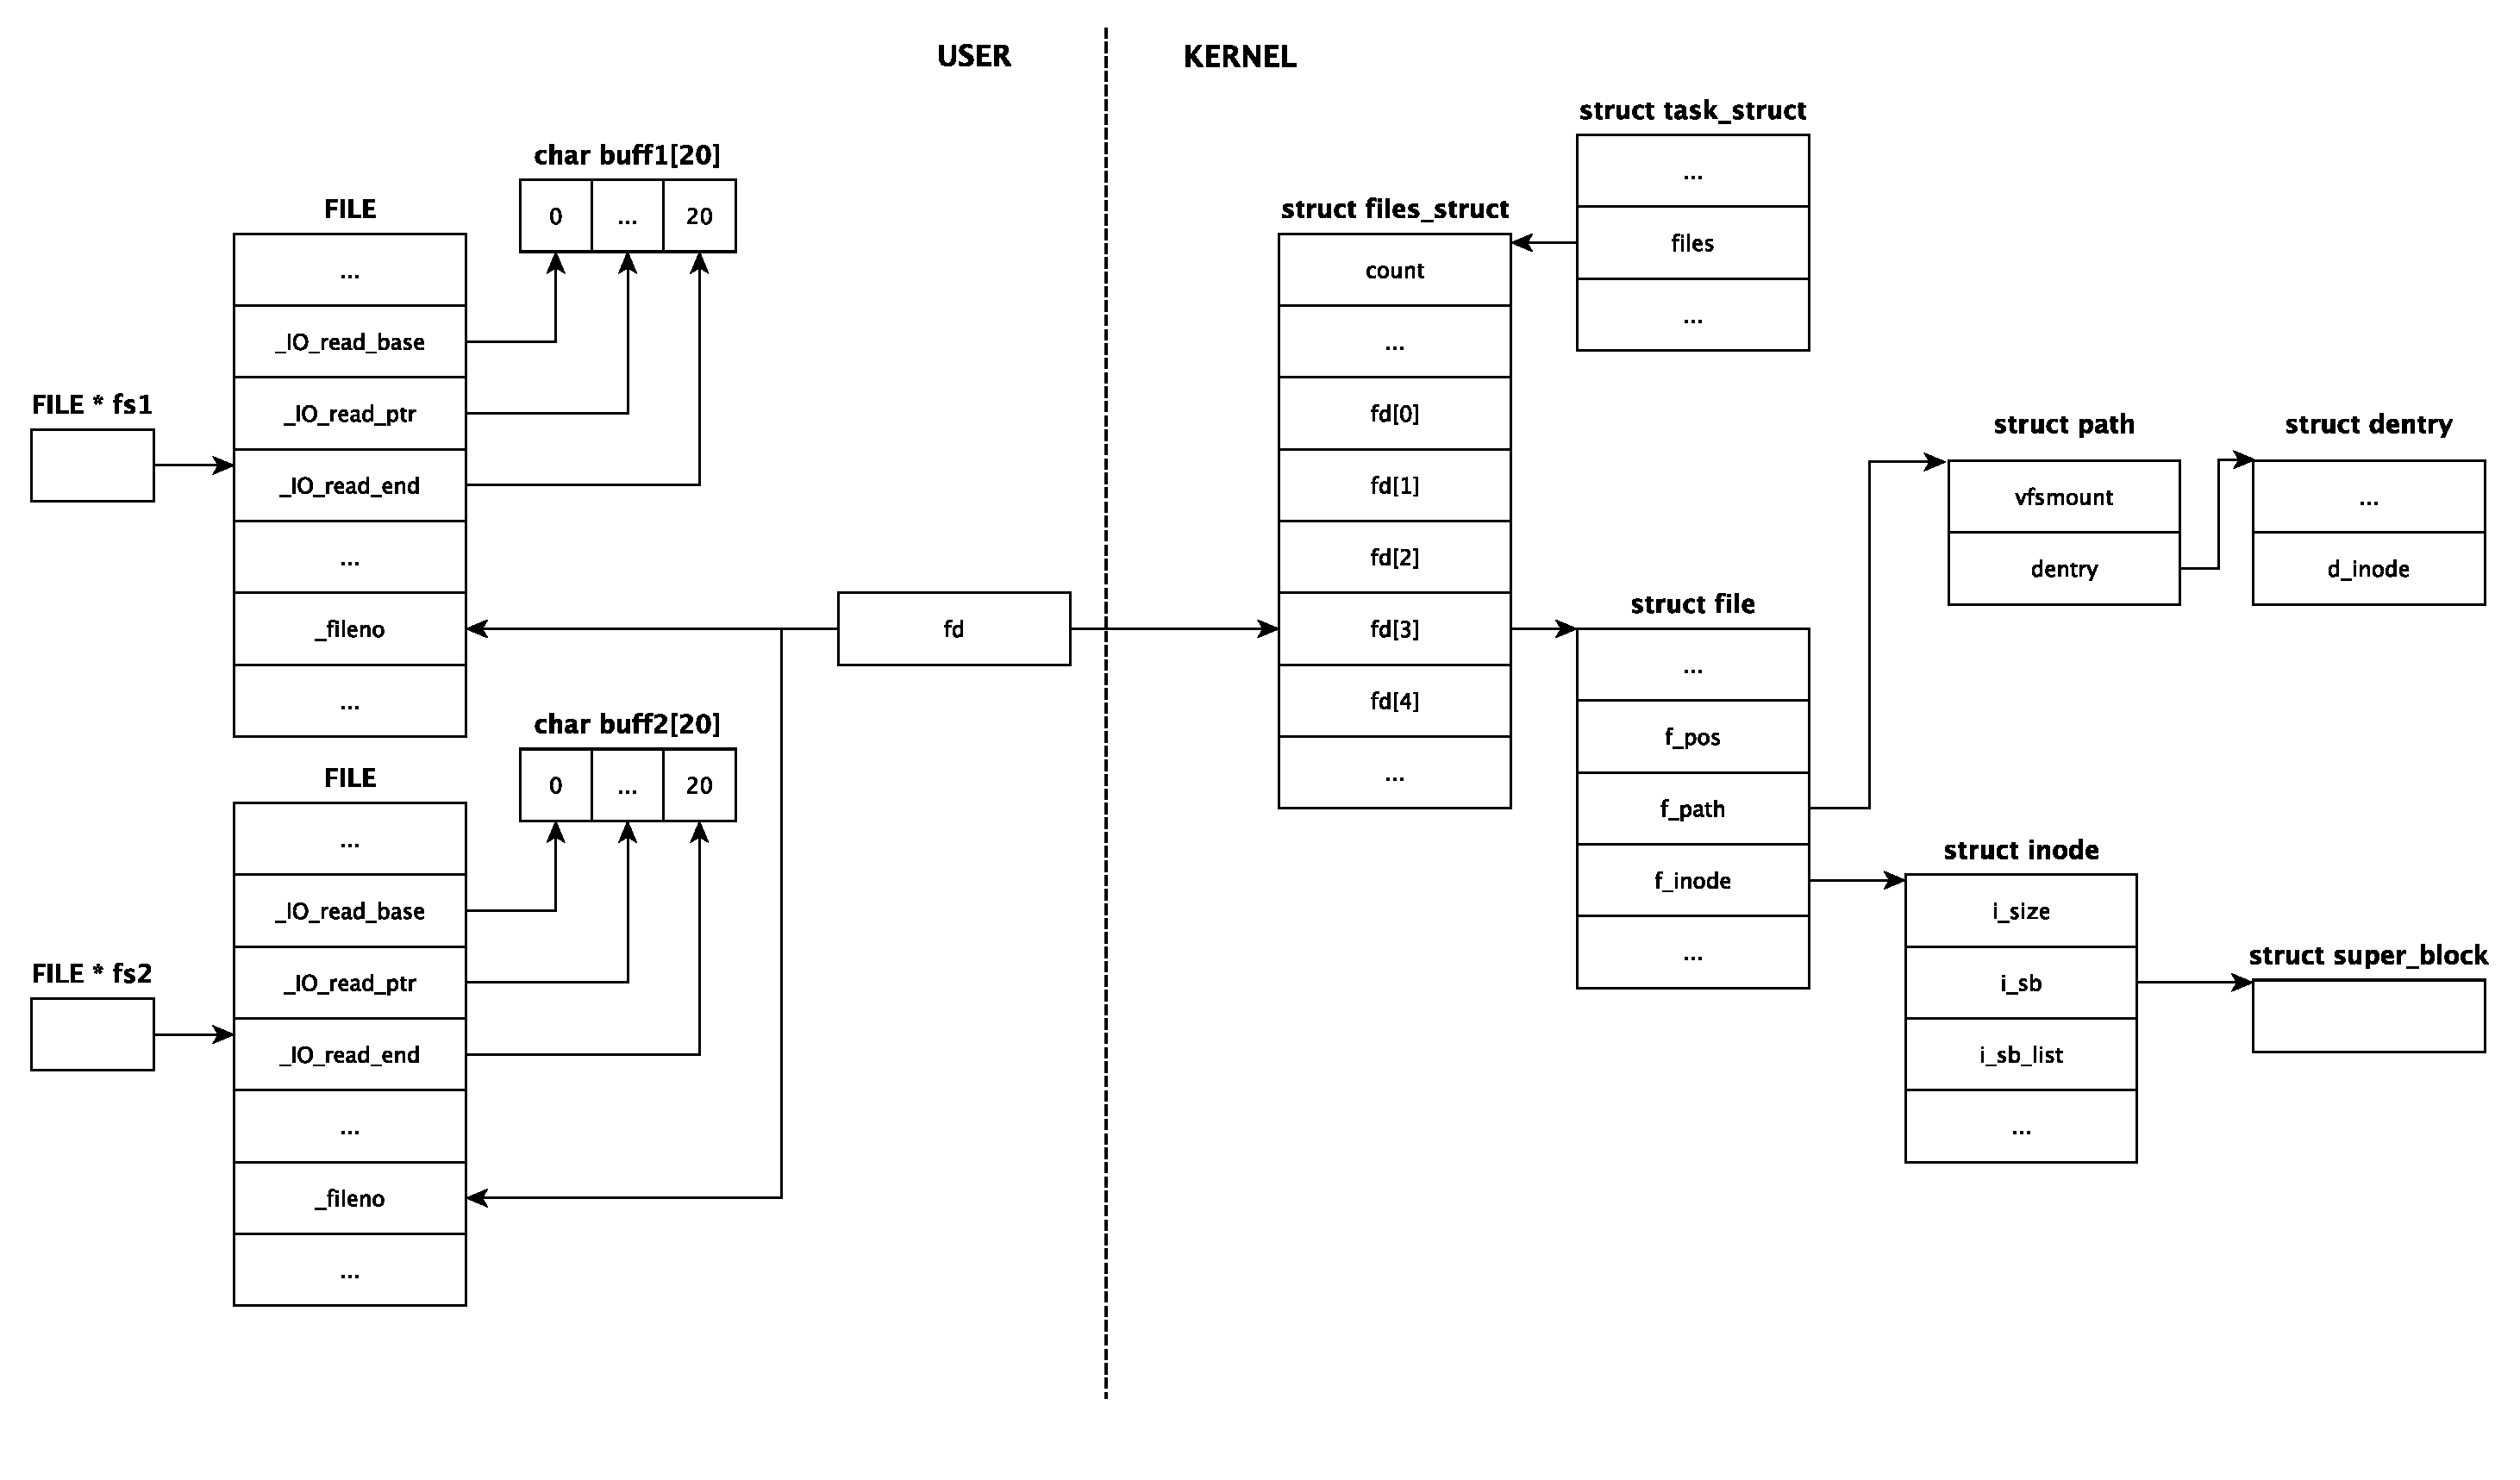
\includegraphics[width=0.9\linewidth]{./images/scheme1.pdf}
		\captionof{figure}{Используемые структуры}
		\label{img:1}
	\end{tabular}
\end{table}

\chapter{Программа 2} 

\section{Однопоточная реализация}

\begin{lstlisting}
	#include <fcntl.h>
#include <unistd.h>

int main()
{
  char c;    

  int fd1 = open("alphabet.txt", O_RDONLY);
  int fd2 = open("alphabet.txt", O_RDONLY);

  while((read(fd1, &c, 1) == 1) && (read(fd2, &c, 1) == 1))
  {
    write(1, &c, 1);
    write(1, &c, 1);
  }

  return 0;
}
\end{lstlisting}

\textbf{Вывод программы}

\begin{lstlisting}
	aabbccddeeffgghhiijjkkllmmnnooppqqrrssttuuvvwwxxyyzz
\end{lstlisting}

\section{Многопоточная реализация}

\begin{lstlisting}
	#include <fcntl.h>
#include <pthread.h>
#include <unistd.h>
#include <stdio.h>

#define BUF_SIZE 20
#define FILENAME "alphabet.txt"

void* thread1()
{
  int fd = open(FILENAME, O_RDONLY);

  char c;
  while ((read(fd, &c, 1)) == 1) write(1, &c, 1);

  return NULL;
}

void* thread2()
{
  int fd = open(FILENAME, O_RDONLY);

  char c;
  while ((read(fd, &c, 1)) == 1) write(1, &c, 1);

  return NULL;
}

int main()
{
  pthread_t t1, t2;

  pthread_create(&t1, NULL, thread1, NULL);
  pthread_create(&t2, NULL, thread2, NULL);

  pthread_join(t1, NULL);
  pthread_join(t2, NULL);

  return 0;
}
\end{lstlisting}

\textbf{Вывод программы на разных запусках}

\begin{lstlisting}
	aabbcdcedfegfhgihjikjlkmlnmonpoqprqsrtsutvuwvxwyxzyz
	aabcbdcedfegfhgihjikjlklmmnnooppqqrrssttuuvvwwxxyyzz
	aabbccddeeffgghhijklmnoipjqkrlsmtnuovpwqxrysztuvwxyz
\end{lstlisting}

\section{Пояснение}

Функция \texttt{open()} два раза создает дескриптор для одного и того же файла в системной таблице открытых файлов, поэтому в программе существует два различных дескриптора открытого файла (\texttt{struct file}), ссылающихся на один	и тот же \texttt{struct inode}.
	
	 Так как у каждой структуры \texttt{struct file} свое поле \texttt{f\_pos}, выводимые символы будут дублироваться.
	
	В случае многопоточной реализации потоки выполняются с разной скоростью,  поэтому символы перемешаются.

\begin{table}[H]
	\centering
	\begin{tabular}{p{1\linewidth}}
		\centering
		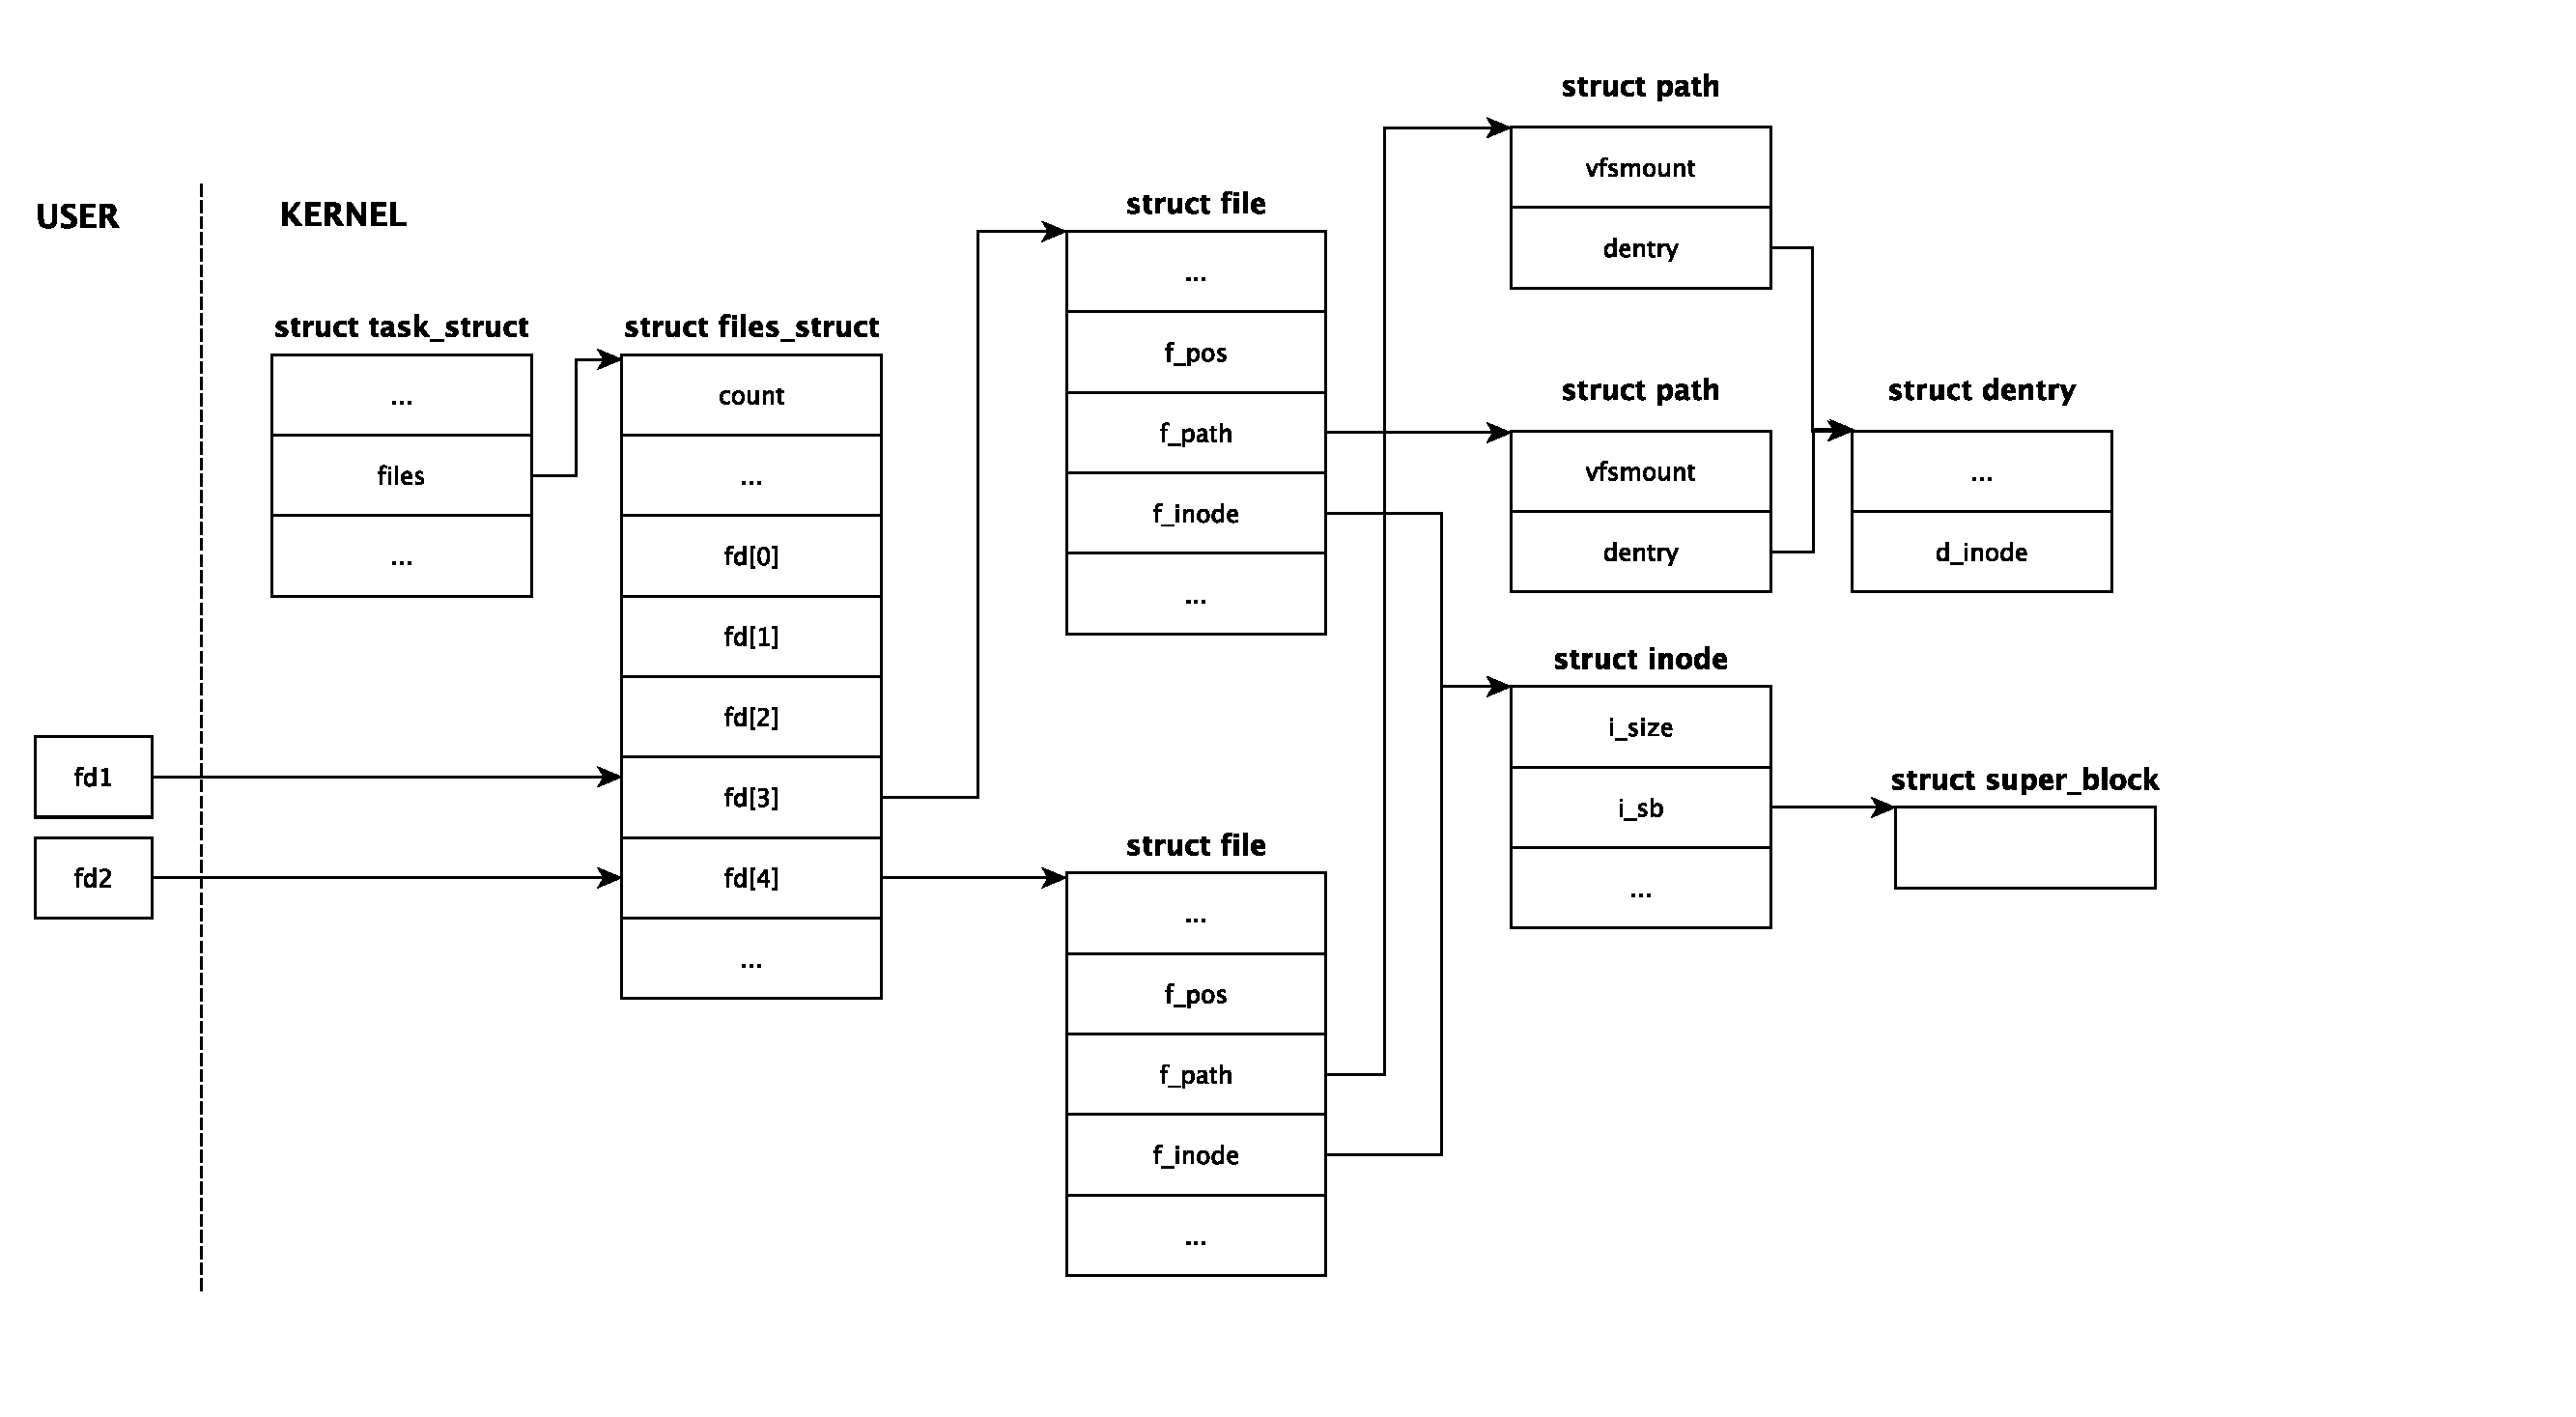
\includegraphics[width=1.0\linewidth]{./images/scheme2.pdf}
		\captionof{figure}{Используемые структуры}
		\label{img:2}
	\end{tabular}
\end{table}

\chapter{Программа 3} 

\section{fopen()}

\section{Однопоточная реализация}

\begin{lstlisting}
#include <fcntl.h>
#include <stdio.h> 
#include <sys/types.h> 
#include <sys/stat.h>
#include <unistd.h>

#define FILENAME "tmp1.txt"

int main()
{
	struct stat buf;

	FILE* f1 = fopen(FILENAME, "w");

	int rc = fstat(f1->_file, &buf);
	if (!rc)
	{
		fprintf(stdout, "after fopen f1: inode - %ju, total size - %lld\n", (uintmax_t)buf.st_ino, buf.st_size);
	}

	FILE* f2 = fopen(FILENAME, "w");

	rc = fstat(f2->_file, &buf);
	if (!rc)
	{
		fprintf(stdout, "after fopen f2: inode - %ju, total size - %lld\n", (uintmax_t)buf.st_ino, buf.st_size);
	}

	for (char c = 'a'; c <= 'z'; c++)
	{
		if (c % 2)
		{
			fprintf(f1, "%c", c);
		}
		else
		{
			fprintf(f2, "%c", c); 
		}
	}

	rc = fstat(f1->_file, &buf);
	if (!rc)
	{
		fprintf(stdout, "before fclose f1: inode - %ju, total size - %lld\n", (uintmax_t)buf.st_ino, buf.st_size);
	}

	rc = fstat(f2->_file, &buf);
	if (!rc)
	{
		fprintf(stdout, "before fclose f2: inode - %ju, total size - %lld\n", (uintmax_t)buf.st_ino, buf.st_size);
	}

	fclose(f1);

	rc = stat(FILENAME, &buf);
	fprintf(stdout, "after fclose f1: inode - %ju, total size - %lld\n", (uintmax_t)buf.st_ino, buf.st_size);

	fclose(f2);

	rc = stat(FILENAME, &buf);
	fprintf(stdout, "after fclose f2: inode - %ju, total size - %lld\n", (uintmax_t)buf.st_ino, buf.st_size);

	return 0;
}
\end{lstlisting}

\textbf{Вывод программы}

\begin{lstlisting}
	bdfhjlnprtvxz
\end{lstlisting}

\textbf{Вывод stat}

\begin{lstlisting}
after open f1: inode - 17875612, total size - 0
after open f2: inode - 17875612, total size - 0
before fclose f1: inode - 17875612, total size - 0
before fclose f2: inode - 17875612, total size - 0
after fclose f1: inode - 17875612, total size - 13
after fclose f2: inode - 17875612, total size - 13
\end{lstlisting}

\section{Многопоточная реализация}

\begin{lstlisting}
	#include <fcntl.h>
#include <pthread.h>
#include <stdio.h>
#include <unistd.h>

#define FILENAME "tmp2.txt"

void* thread1()
{
  FILE* f = fopen(FILENAME, "w");

  for (char c = 'a'; c <= 'z'; c += 2)
  {
    fprintf(f, "%c", c);
  }

  fclose(f);

  return NULL;
}

void* thread2() 
{
  FILE* f = fopen(FILENAME, "w");

  for (char c = 'b'; c <= 'z'; c += 2)
  { 
    fprintf(f, "%c", c);
  }

  fclose(f);

  return NULL;
}

int main()
{
  pthread_t t1, t2;

  pthread_create(&t1, NULL, thread1, NULL);
  pthread_create(&t2, NULL, thread2, NULL);

  pthread_join(t1, NULL);
  pthread_join(t2, NULL);

  return 0;
}
\end{lstlisting}

\textbf{Вывод программы на разных запусках}

\begin{lstlisting}
	acegikmoqsuwy
	bdfhjlnprtvxz
\end{lstlisting}

\section{Пояснение}

 Файл открывается на запись два раза функцией \texttt{fopen()}, которая внутри своего кода вызывает \texttt{open()}. Каждое открытие файла сопровождается созданием дескриптора открытого файла \texttt{struct file}, содержащего поле f\_pos.
 
  Поля \texttt{f\_pos} двух разных дескрипторов одного открытого файла независимы, поэтому запись в файл будет производится с нулевой позиции.

Функция \texttt{fprintf()} предоставляет буферизованный вывод, поэтому сначала информация пишется в буфер, а из буфера в файл при одном из условий:
\begin{enumerate}
	\item буфер заполнен;
	\item вызвана функция \texttt{fclose()};
	\item вызвана функция \texttt{fflush()} (принудительная запись).
\end{enumerate}

При вызове \texttt{fclose()} для fs1 буфер для fs1 записывается в файл. При вызове \texttt{fclose()} для fs2, все содержимое файла затирается, а в файл записывается содержимое буфера для fs2. В итоге произошла потеря данных, в файле окажется только содержимое буфера для fs2. 

Чтобы этого избегать, необходимо использовать флаг O\_APPEND. Если этот флаг установлен, то первая запись в файл не теряется. 

В случае многопоточной реализации потоки выполняются с разной скоростью,  поэтому символы перемешаются.

\begin{table}[H]
	\centering
	\begin{tabular}{p{1\linewidth}}
		\centering
		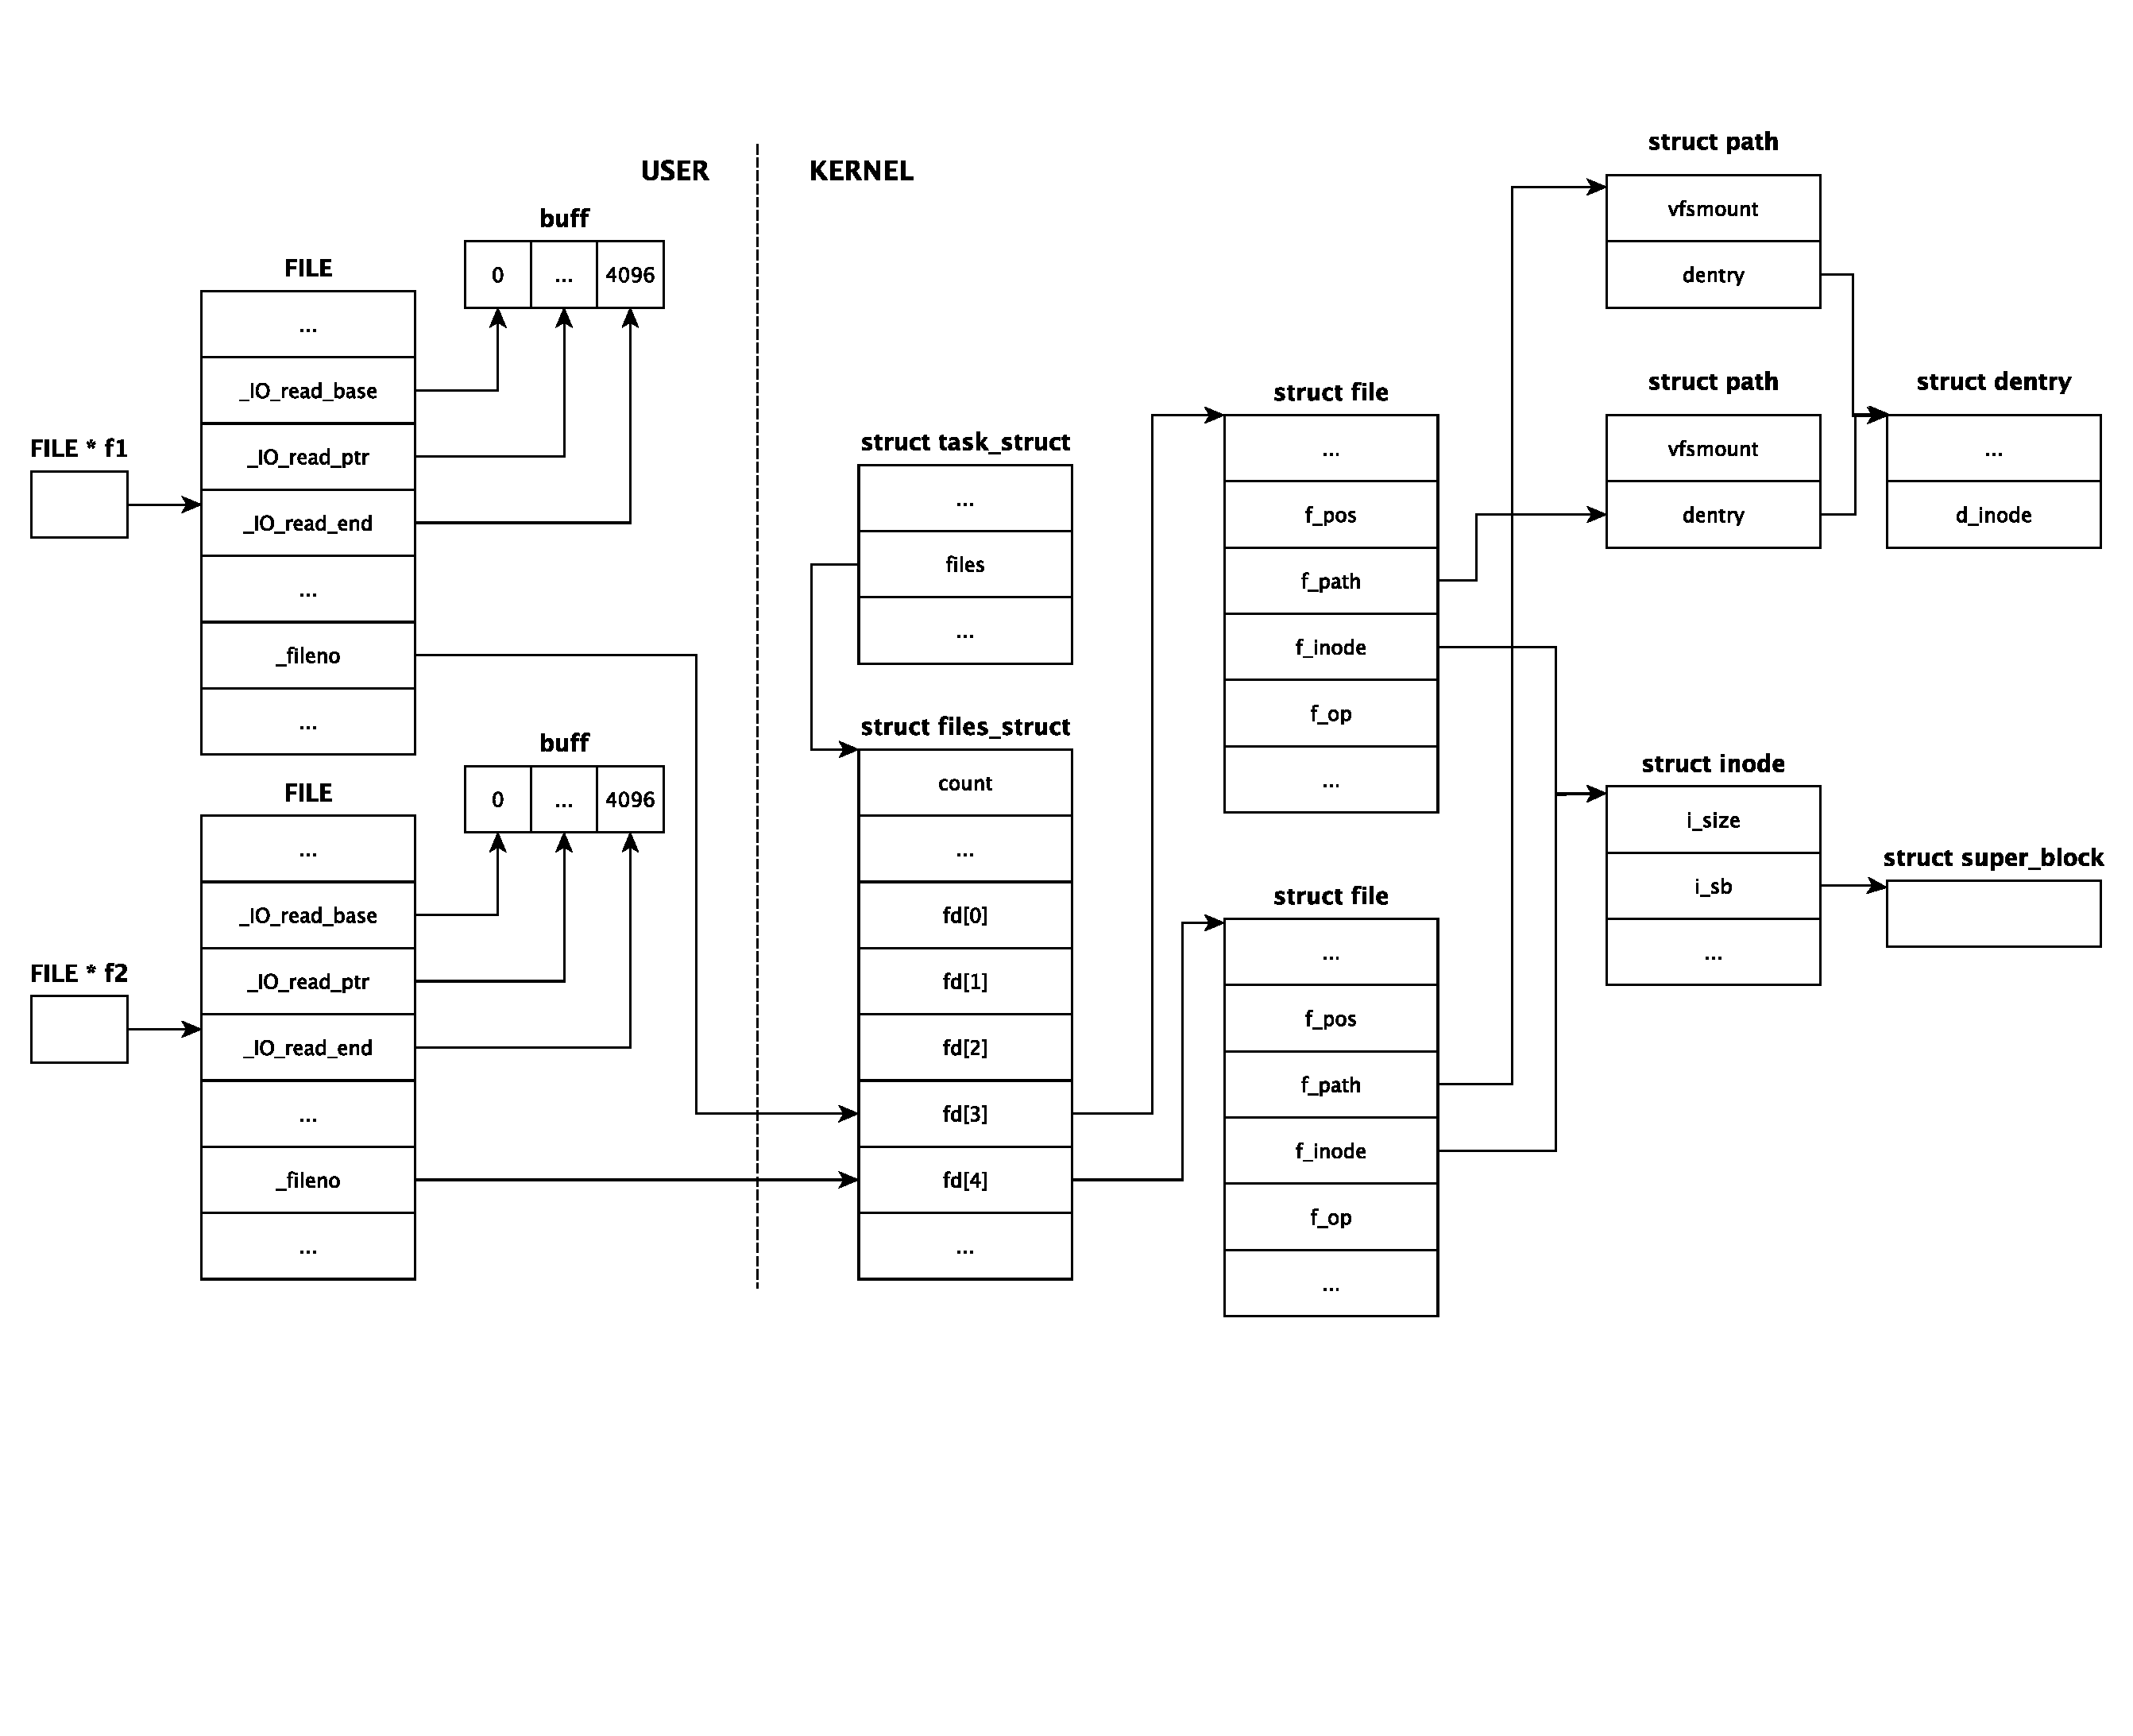
\includegraphics[width=0.8\linewidth]{./images/scheme3.pdf}
		\captionof{figure}{Используемые структуры}
		\label{img:3}
	\end{tabular}
\end{table}

\section{open()}

\section{Однопоточная реализация}

\begin{lstlisting}
#include <fcntl.h>
#include <stdio.h> 
#include <sys/types.h> 
#include <sys/stat.h>
#include <unistd.h>

#define FILENAME "tmp3.txt"

int main()
{
	struct stat buf;

	int f1 = open(FILENAME, O_WRONLY | O_CREAT, S_IRUSR | S_IWUSR);

	int rc = fstat(f1, &buf);
	if (!rc)
	{
		fprintf(stdout, "after open f1: inode - %ju, total size - %lld\n", (uintmax_t)buf.st_ino, buf.st_size);
	}

	int f2 = open(FILENAME, O_WRONLY | O_CREAT, S_IRUSR | S_IWUSR);

	rc = fstat(f2, &buf);
	if (!rc)
	{
		fprintf(stdout, "after open f2: inode - %ju, total size - %lld\n", (uintmax_t)buf.st_ino, buf.st_size);
	}

	for (char c = 'a'; c <= 'z'; c++)
	{
		if (c % 2)
		{
			write(f1, &c, 1);
		}
		else
		{
			write(f2, &c, 1); 
		}
	}

	rc = fstat(f1, &buf);
	if (!rc)
	{
		fprintf(stdout, "before close f1: inode - %ju, total size - %lld\n", (uintmax_t)buf.st_ino, buf.st_size);
	}
	rc = fstat(f2, &buf);
	if (!rc)
	{
		fprintf(stdout, "before close f2: inode - %ju, total size - %lld\n", (uintmax_t)buf.st_ino, buf.st_size);
	}

	close(f1);

	rc = stat(FILENAME, &buf);
	fprintf(stdout, "after close f1: inode - %ju, total size - %lld\n", (uintmax_t)buf.st_ino, buf.st_size);

	close(f2);

	rc = stat(FILENAME, &buf);
	fprintf(stdout, "after fclose f2: inode - %ju, total size - %lld\n", (uintmax_t)buf.st_ino, buf.st_size);

	return 0;
}
\end{lstlisting}

\textbf{Вывод программы}

\begin{lstlisting}
	bdfhjlnprtvxz
\end{lstlisting}

\textbf{Вывод stat}

\begin{lstlisting}
after open f1: inode - 17885541, total size - 0
after open f2: inode - 17885541, total size - 0
before close f1: inode - 17885541, total size - 13
before close f2: inode - 17885541, total size - 13
after close f1: inode - 17885541, total size - 13
after fclose f2: inode - 17885541, total size - 13
\end{lstlisting}

\section{Многопоточная реализация}

\begin{lstlisting}
	#include <fcntl.h>
#include <pthread.h>
#include <stdio.h>
#include <unistd.h>

#define FILENAME "tmp4.txt"

void* thread1()
{
  int f = open(FILENAME, O_WRONLY | O_CREAT, S_IRUSR | S_IWUSR);

  for (char c = 'a'; c <= 'z'; c += 2)
  {
    write(f, &c, 1);
  }

  close(f);

  return NULL;
}

void* thread2() 
{
  int f = open(FILENAME, O_WRONLY | O_CREAT, S_IRUSR | S_IWUSR);

  for (char c = 'b'; c <= 'z'; c += 2)
  { 
    write(f, &c, 1);
  }

  close(f);

  return NULL;
}

int main()
{
  pthread_t t1, t2;
  pthread_create(&t1, NULL, thread1, NULL);
  pthread_create(&t2, NULL, thread2, NULL);

  pthread_join(t1, NULL);
  pthread_join(t2, NULL);

  return 0;
}
\end{lstlisting}

\textbf{Вывод программы на разных запусках}

\begin{lstlisting}
	bdfhjlnprtvxz
	acegikmoqsuwy
\end{lstlisting}

\section{open() + O\_APPEND}

\section{Однопоточная реализация}

\begin{lstlisting}
#include <fcntl.h>
#include <stdio.h> 
#include <sys/types.h> 
#include <sys/stat.h>
#include <unistd.h>

#define FILENAME "tmp5.txt"

int main()
{
	struct stat buf;

	int f1 = open(FILENAME, O_WRONLY | O_CREAT | O_APPEND, S_IRUSR | S_IWUSR);

	int rc = fstat(f1, &buf);
	if (!rc)
	{
		fprintf(stdout, "after open f1: inode - %ju, total size - %lld\n", (uintmax_t)buf.st_ino, buf.st_size);
	}

	int f2 = open(FILENAME, O_WRONLY | O_CREAT | O_APPEND, S_IRUSR | S_IWUSR);

	rc = fstat(f2, &buf);
	if (!rc)
	{
		fprintf(stdout, "after open f2: inode - %ju, total size - %lld\n", (uintmax_t)buf.st_ino, buf.st_size);
	}

	for (char c = 'a'; c <= 'z'; c++)
	{
		if (c % 2)
		{
			write(f1, &c, 1);
		}
		else
		{
			write(f2, &c, 1); 
		}
	}

	rc = fstat(f1, &buf);
	if (!rc)
	{
		fprintf(stdout, "before close f1: inode - %ju, total size - %lld\n", (uintmax_t)buf.st_ino, buf.st_size);
	}

	rc = fstat(f2, &buf);
	if (!rc)
	{
		fprintf(stdout, "before close f2: inode - %ju, total size - %lld\n", (uintmax_t)buf.st_ino, buf.st_size);
	}

	close(f1);

	rc = stat(FILENAME, &buf);
	fprintf(stdout, "after close f1: inode - %ju, total size - %lld\n", (uintmax_t)buf.st_ino, buf.st_size);

	close(f2);

	rc = stat(FILENAME, &buf);
	fprintf(stdout, "after fclose f2: inode - %ju, total size - %lld\n", (uintmax_t)buf.st_ino, buf.st_size);

	return 0;
}
\end{lstlisting}

\textbf{Вывод программы}

\begin{lstlisting}
	abcdefghijklmnopqrstuvwxyz
\end{lstlisting}

\section{Многопоточная реализация}

\begin{lstlisting}
	#include <fcntl.h>
#include <pthread.h>
#include <stdio.h>
#include <unistd.h>

#define FILENAME "tmp6.txt"

void* thread1()
{
  int f = open(FILENAME, O_WRONLY | O_CREAT | O_APPEND,
  S_IRUSR | S_IWUSR);

  for (char c = 'a'; c <= 'z'; c += 2)
  {
    write(f, &c, 1);
  }

  close(f);

  return NULL;
}

void* thread2() 
{
  int f = open(FILENAME, O_WRONLY | O_CREAT | O_APPEND,
  S_IRUSR | S_IWUSR);

  for (char c = 'b'; c <= 'z'; c += 2)
  { 
    write(f, &c, 1);
  }

  close(f);

  return NULL;
}

int main()
{
  pthread_t t1, t2;

  pthread_create(&t1, NULL, thread1, NULL);
  pthread_create(&t2, NULL, thread2, NULL);

  pthread_join(t1, NULL);
  pthread_join(t2, NULL);

  return 0;
}
\end{lstlisting}

\textbf{Вывод программы на разных запусках}

\begin{lstlisting}
	acbdefghijklmnopqrstuvwxyz
	abcdfehgjilknmporqtsvuxwzy
\end{lstlisting}

\textbf{Вывод stat}

\begin{lstlisting}
after open f1: inode - 17888251, total size - 0
after open f2: inode - 17888251, total size - 0
before close f1: inode - 17888251, total size - 26
before close f2: inode - 17888251, total size - 26
after close f1: inode - 17888251, total size - 26
after fclose f2: inode - 17888251, total size - 26
\end{lstlisting}

\section{Пояснение}
Если указан флаг O\_APPEND, файл открывается в режиме добавления (записи в конец файла). Перед каждой операцией write файловый указатель будет устанавливаться в конце файла, как если бы использовался \texttt{lseek()}. Если этот флаг установлен, первая запись в файл не теряется.

\chapter{Заключение}
Таким образом, при буферизованном вводе-выводе все данные и при чтении, и при записи пишутся сначала в буфер, а только после этого в файл. При отсутствии буферизации данные сразу пишутся в/читаются из файла. 

В программе с \texttt{fopen()}, \texttt{fprintf()} (с буферизацией) содержимое файла затирается при вызове \texttt{fclose()}. Поэтому размер файла до вызова \texttt{fclose()} по данным из \texttt{stat()} равен 0.

В программе с \texttt{open()}, \texttt{write()} (без буферизации) содержимое файла затирается при вызове \texttt{write()}. Поэтому размер файла до вызова \texttt{fclose()} по данным из \texttt{stat()} равен 13~---~столько символов в итоге останется в файле.





